\documentclass[tikz, border=5mm]{standalone}
\usepackage{amsmath}
\usetikzlibrary{positioning, shapes.geometric, arrows.meta, fit, backgrounds, calc}
\begin{document}
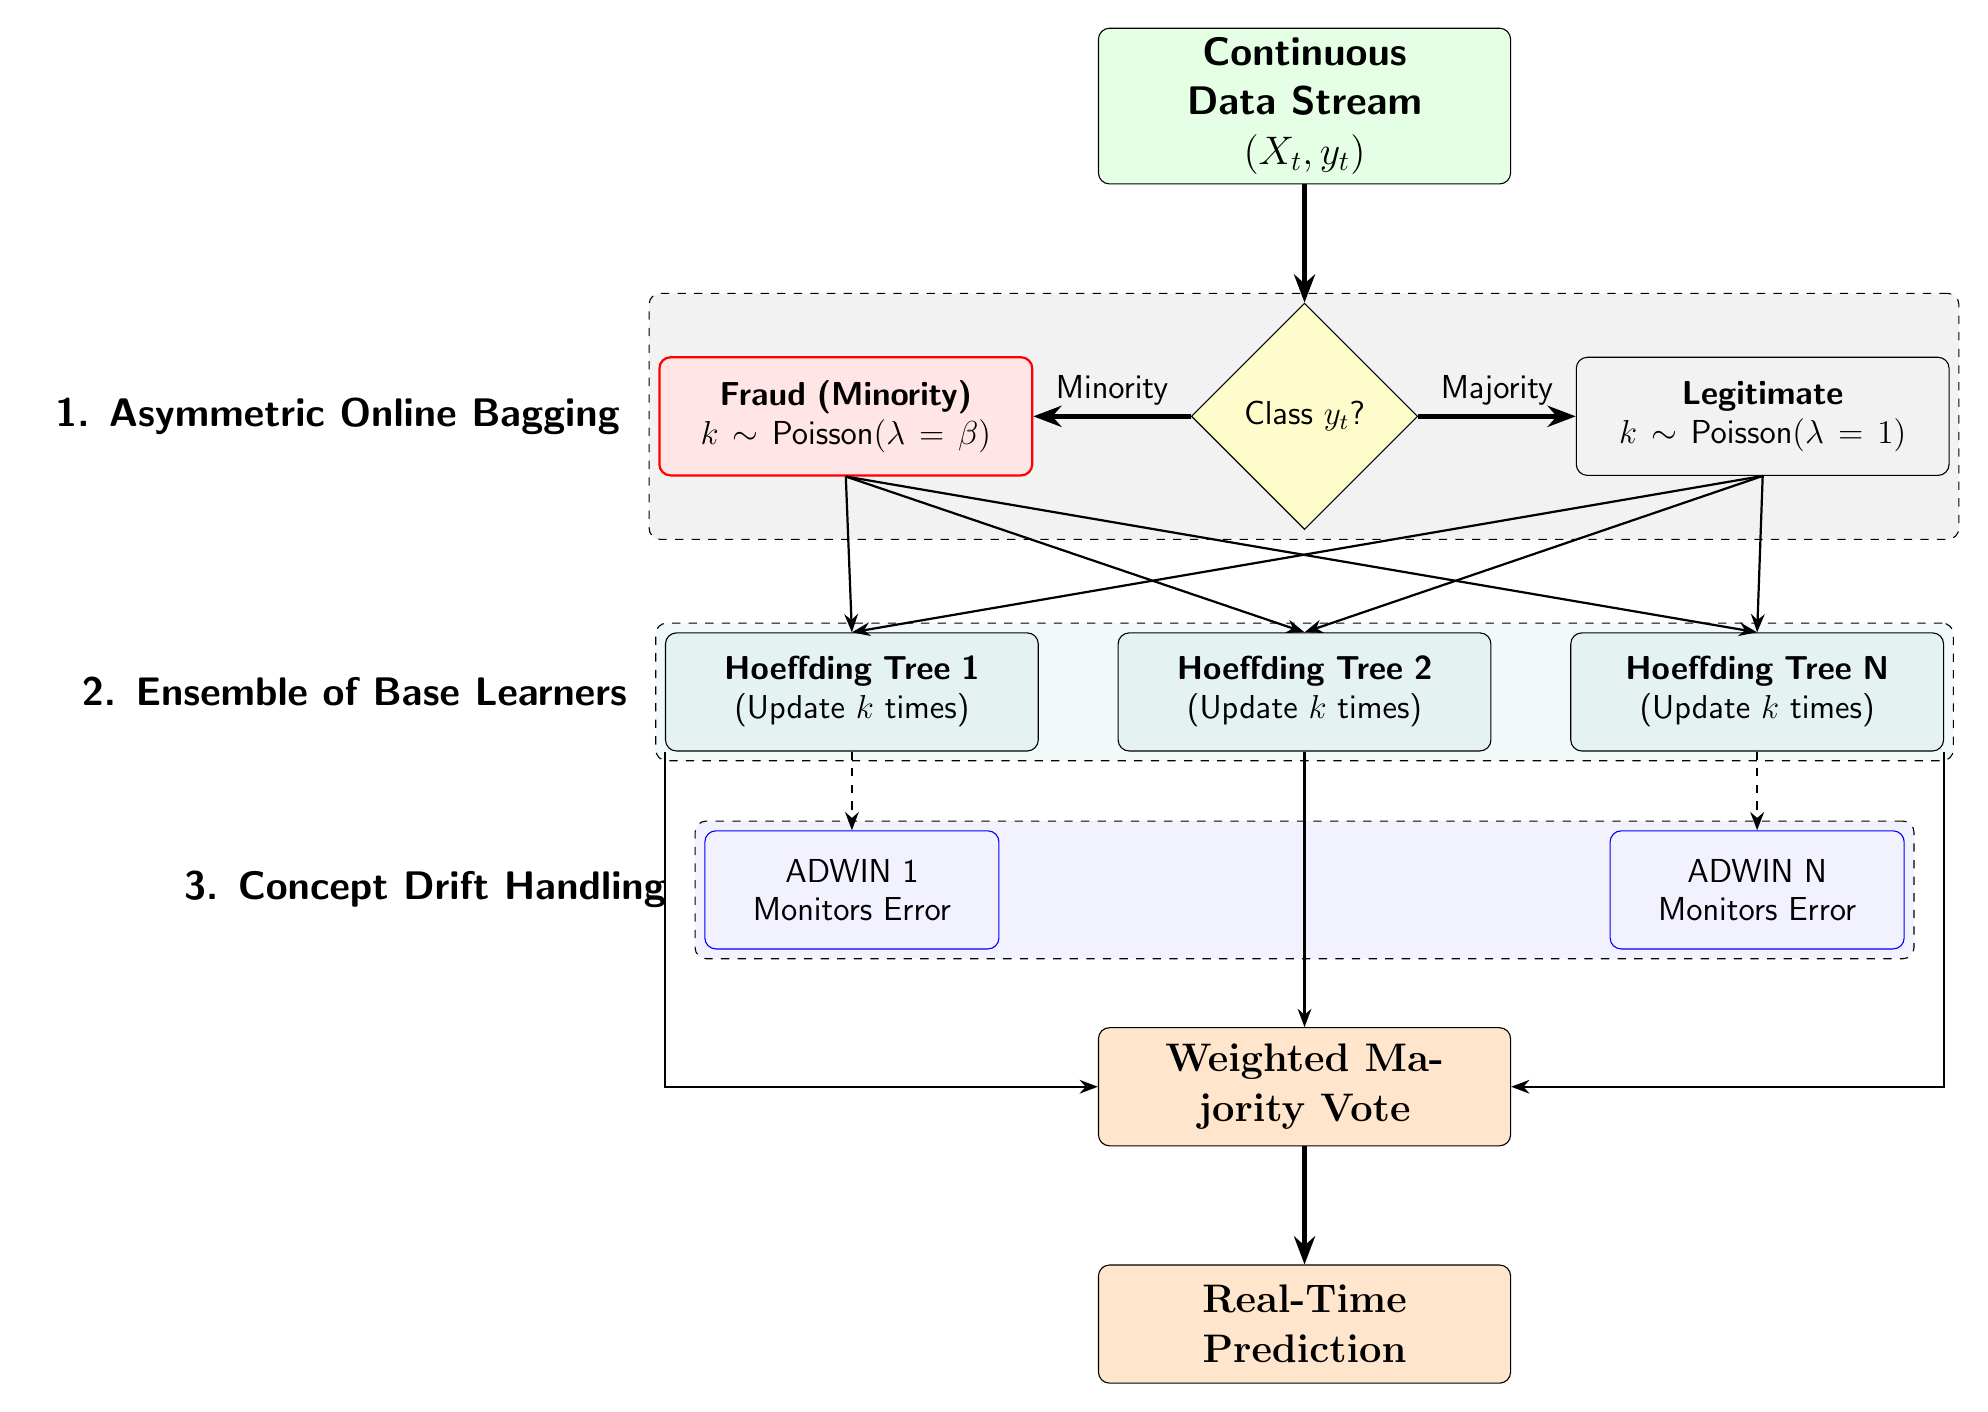
\begin{tikzpicture}[
    font=\sffamily\large,
    >=Stealth,
    node distance=1.5cm and 2cm,
    block/.style={rectangle, draw, fill=blue!10, rounded corners, text width=4cm, text centered, minimum height=1.5cm},
    decision/.style={diamond, draw, fill=yellow!20, text width=2.5cm, text badly centered, inner sep=0pt},
    stream/.style={rectangle, draw, fill=green!10, text width=5cm, text centered, minimum height=1.5cm, rounded corners, font=\sffamily\Large\bfseries},
    fraud/.style={rectangle, draw=red, thick, fill=red!10, rounded corners, text width=4.5cm, text centered, minimum height=1.5cm},
    legit/.style={rectangle, draw=black, fill=gray!10, rounded corners, text width=4.5cm, text centered, minimum height=1.5cm},
    tree/.style={rectangle, draw, fill=teal!10, rounded corners, text width=4.5cm, text centered, minimum height=1.5cm},
    monitor/.style={rectangle, draw=blue, fill=blue!5, rounded corners, text width=3.5cm, text centered, minimum height=1.5cm},
    output/.style={rectangle, draw, fill=orange!20, rounded corners, text width=5cm, text centered, minimum height=1.5cm, font=\Large\bfseries}
]

% 1. Input (Top)
\node[stream] (input) {Continuous Data Stream \\ $(X_t, y_t)$};

% 2. Asymmetric Bagging (Below Input)
\node[decision, below=1.5cm of input] (check) {Class $y_t$?};
\node[fraud, left=2cm of check] (poisson1) {\textbf{Fraud (Minority)} \\ $k \sim \text{Poisson}(\lambda=\beta)$};
\node[legit, right=2cm of check] (poisson2) {\textbf{Legitimate} \\ $k \sim \text{Poisson}(\lambda=1)$};

% 3. Trees (Below Bagging)
\coordinate (centerTree) at ($(check) + (0, -3.5)$);
\node[tree] at (centerTree) (tree2) {\textbf{Hoeffding Tree 2} \\ (Update $k$ times)};
\node[tree, left=1cm of tree2] (tree1) {\textbf{Hoeffding Tree 1} \\ (Update $k$ times)};
\node[tree, right=1cm of tree2] (tree3) {\textbf{Hoeffding Tree N} \\ (Update $k$ times)};

% 4. ADWIN (Below Trees)
\node[monitor, below=1cm of tree1] (adwin1) {ADWIN 1 \\ Monitors Error};
\node[monitor, below=1cm of tree3] (adwin3) {ADWIN N \\ Monitors Error};

% 5. Voting & Output (Bottom)
\node[output, below=3.5cm of tree2] (vote) {Weighted Majority Vote};
\node[output, below=1.5cm of vote] (final) {Real-Time Prediction};

% Paths
\draw[->, ultra thick] (input) -- (check);
\draw[->, ultra thick] (check) -- node[above] {Minority} (poisson1);
\draw[->, ultra thick] (check) -- node[above] {Majority} (poisson2);

\draw[->, thick] (poisson1.south) -- (tree1.north);
\draw[->, thick] (poisson1.south) -- (tree2.north);
\draw[->, thick] (poisson1.south) -- (tree3.north);

\draw[->, thick] (poisson2.south) -- (tree1.north);
\draw[->, thick] (poisson2.south) -- (tree2.north);
\draw[->, thick] (poisson2.south) -- (tree3.north);

\draw[->, dashed, thick] (tree1.south) -- (adwin1.north);
\draw[->, dashed, thick] (tree3.south) -- (adwin3.north);

\draw[->, thick] (tree1.south west) |- (vote.west);
\draw[->, thick] (tree2.south) -- (vote.north);
\draw[->, thick] (tree3.south east) |- (vote.east);

\draw[->, ultra thick] (vote) -- (final);

% Backgrounds
\begin{scope}[on background layer]
    \node[draw, dashed, rounded corners, fit=(check) (poisson1) (poisson2), fill=gray!10, label={[anchor=east, inner sep=10pt]180:\Large\textbf{1. Asymmetric Online Bagging}}] (group1) {};
    \node[draw, dashed, rounded corners, fit=(tree1) (tree3), fill=teal!5, label={[anchor=east, inner sep=10pt]180:\Large\textbf{2. Ensemble of Base Learners}}] (group2) {};
    \node[draw, dashed, rounded corners, fit=(adwin1) (adwin3), fill=blue!5, label={[anchor=east, inner sep=10pt]180:\Large\textbf{3. Concept Drift Handling}}] (group3) {};
\end{scope}

\end{tikzpicture}
\end{document}
